% !TeX root = ../Main-Report.tex

\chapter{Forward and Inverse Kinematics}


\section{Forward Kinematics}
Calculating forward kinematics is the process of determining the endeffector position depending on the joint variables. The equations for calculating the forward kinematics as well as the needed dimensions of the Delta robot have been taken from \cite{delta_kin} and were put inside a MATLAB-function block to be usable inside Simulink. The code of the function block can be found in \textit{forward\_kinematics.m}.

To be able to verify if the equations have been implemented correctly, the euclidean error between the Multibody simulation (MB) and the output of the forward kinematics function (FK) has been calculated. The results can be seen in figure \ref{fig:fwkinverification}.

% TODO: \usepackage{graphicx} required
\begin{figure}[H]
	\centering
	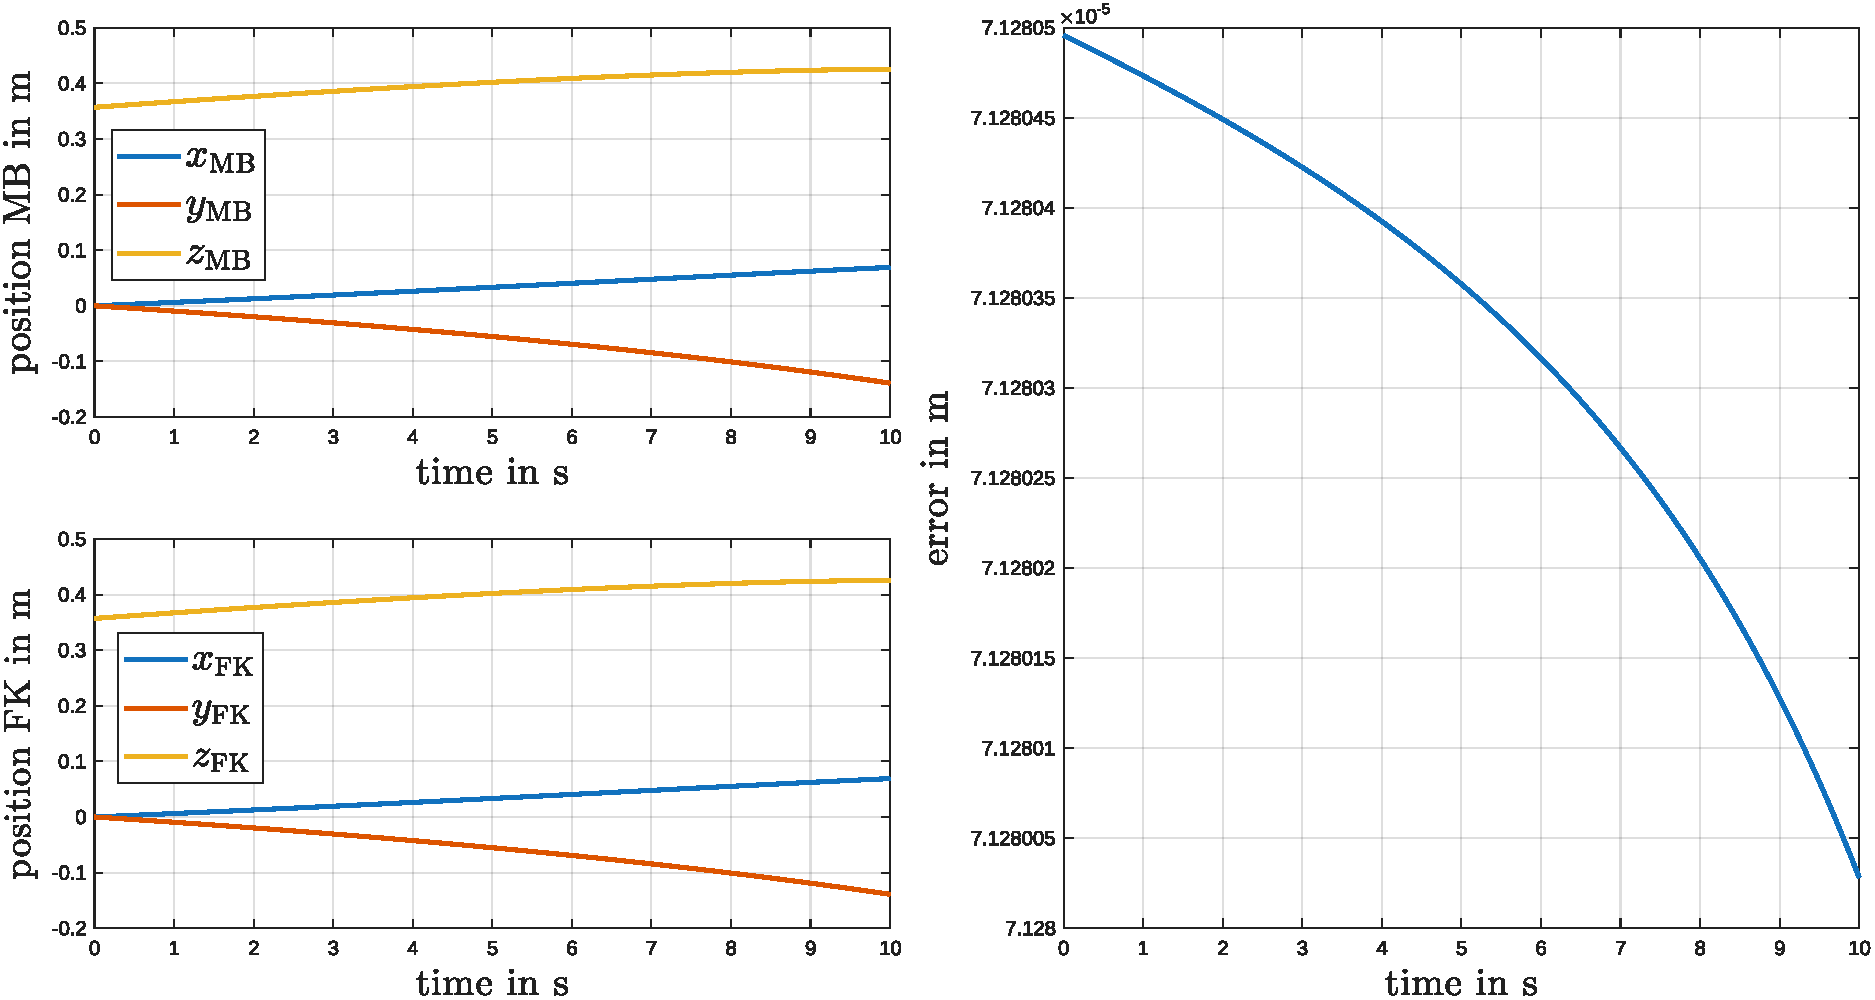
\includegraphics[width=1.0\linewidth]{cus_imgs/fw_kin_verification2}
	\caption[Plot of verification process for forward kinematics]{Plot of Verification process for forward kinematics. Left column: position calculated by Multibody model (MB) and function (FK); right column: euclidean error of the two}
	\label{fig:fwkinverification}
\end{figure}

The left column shows that for the joint trajectory that has been given to the system, the position of the end-effector in simulation and the forward kinematics function yield the same result. The plot in the right column shows an error of magnitudes of $10^{-5}\,\si{\meter}$, which is neglectable.

\section{Inverse Kinematics}
Calculating inverse kinematics is the process of determining the joint positions necessary for the end-effector to be at a given position. The equations for inverse kinematics for the robot are also taken from \cite{delta_kin}. A function called \textit{inverse\_kinematics.m} has been implemented to do the conversion. To verify the results, the end-effector output of the  Multibody-model has been fed into the inverse kinematics function, whose output has been compared to the input into the Simulation. Like above, the inputs are three ramps with different inclinations. The results can be seen in figure \ref{fig:inkinverification}.
\begin{figure}[H]
	\centering
	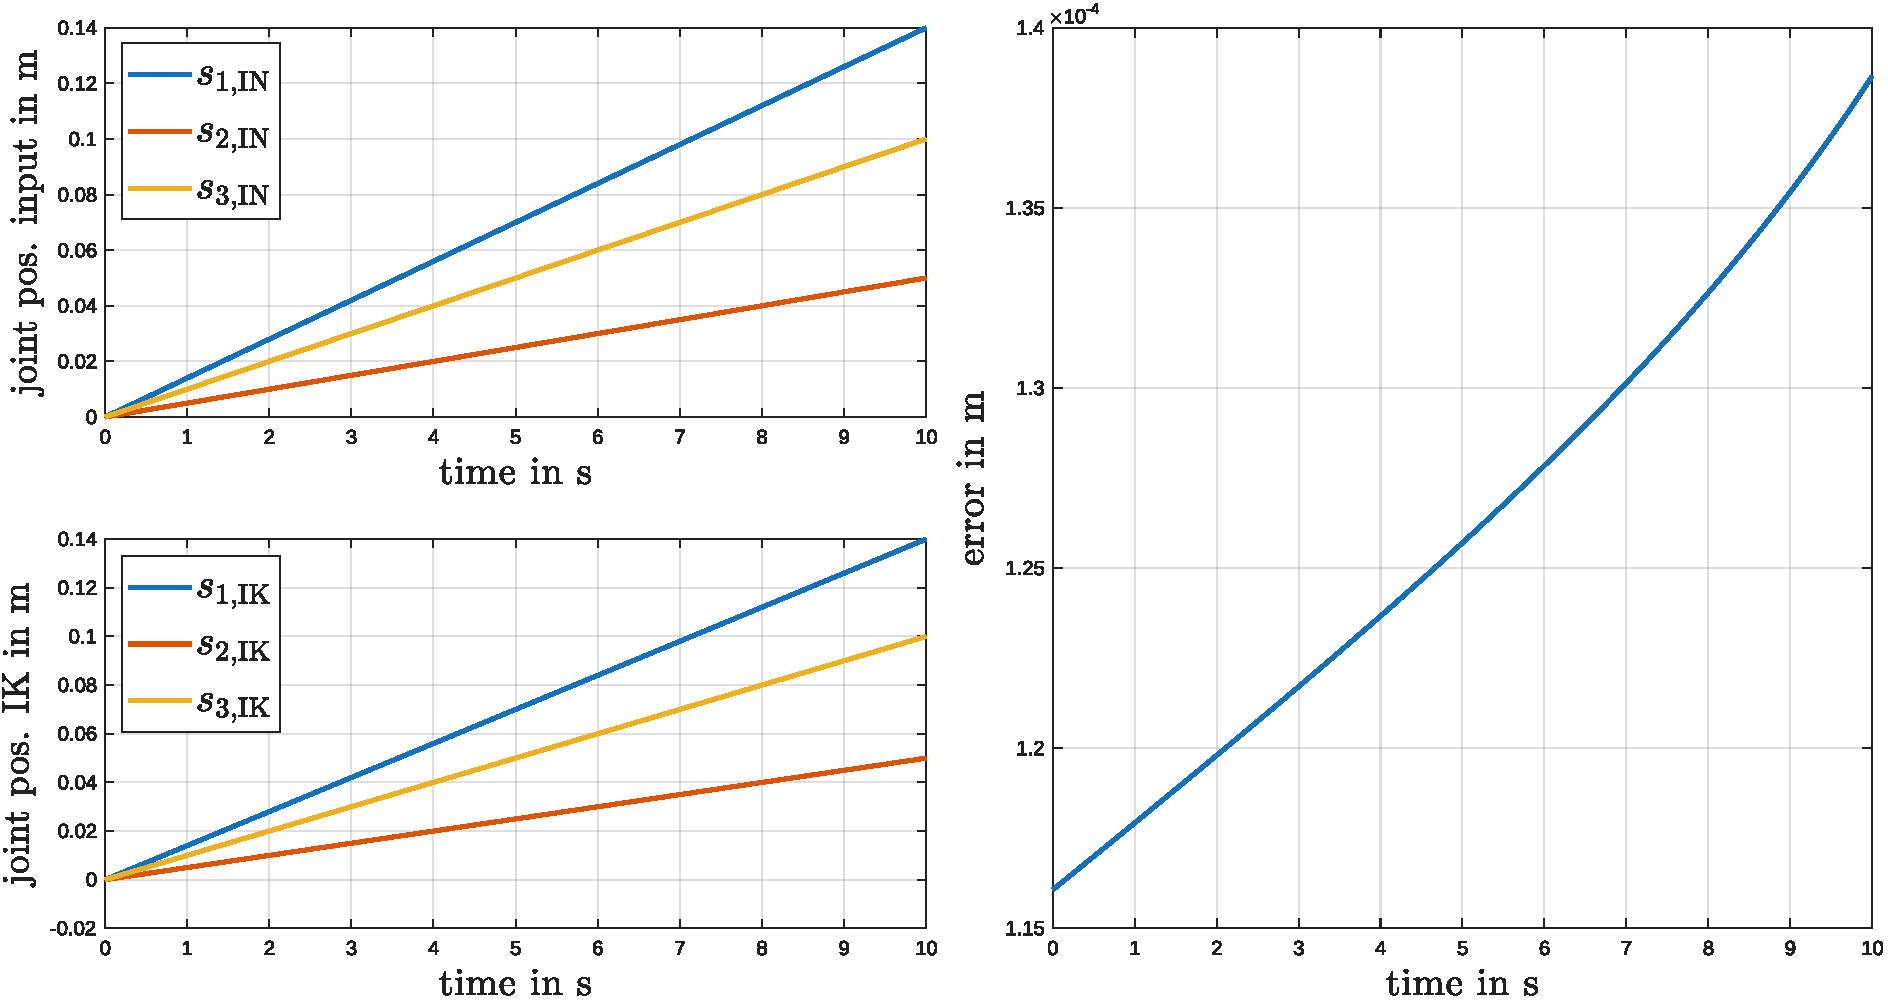
\includegraphics[width=1.0\linewidth]{cus_imgs/in_kin_verification}
	\caption[Plot of verification process for inverse kinematics]{Plot of Verification process for inverse kinematics. Left column: input joint position into Multibody model (MB) and output of inverse kinematics function (IK); right column: euclidean error of the two}
	\label{fig:inkinverification}
\end{figure}

It is apparent, that the inverse kinematics (IK) function yields the same results as the joint positions that were input into the simulation. The error, however, has a magnitude of $10^{-4}\,\si{\meter}$, which is larger than for forward kinematics.